% !TEX TS-program = pdflatex
% !TEX encoding = UTF-8 Unicode

\documentclass[preprint]{sigplanconf}

\usepackage{graphicx,listings,fixltx2e,lambda,array,multirow,color}


\begin{document}
\conferenceinfo{ICFP 2011}{September 19--21, 2011, Tokyo, Japan.}
\copyrightyear{2011}

\preprintfooter{ICFP 2011}
\titlebanner{DRAFT---Do not distribute}

\title{Parakeet: Automatic GPU Acceleration of Dynamic Array Languages}

\authorinfo{Alex Rubinsteyn}{alexr@cs.nyu.edu}{New York University}
\authorinfo{Eric Hielscher}{hielscher@cs.nyu.edu}{New York University}
\authorinfo{Dennis Shasha}{shasha@cs.nyu.edu}{New York University}
\lstset{ 
basicstyle=\small\footnotesize\ttfamily, % Standardschrift
numbers=left,                   % where to put the line-numbers
stepnumber=1,                   % the step between two line-numbers. If it's 1 each line 
numbersep=12pt,                  % how far the line-numbers are from the code
showspaces=false,               % show spaces adding particular underscores
showstringspaces=false,         % underline spaces within strings
showtabs=false,                 % show tabs within strings adding particular underscores
tabsize=2,	                % sets default tabsize to 2 spaces
captionpos=b,                   % sets the caption-position to bottom
breaklines=true,                % sets automatic line breaking
breakatwhitespace=false,        % sets if automatic breaks should only happen at whitespace
keywordstyle=\color{black}\bf,
morekeywords={til,sum,sqrt,all, min, each, where, while,+,*,-,avg},            % if you want to add more keywords to the set
moredelim=[is][\itshape]{/*}{*/},
linewidth={\textwidth},
xleftmargin=20pt,
%framexleftmargin=17pt,
%framexrightmargin=5pt,
%framexbottommargin=4pt,
}

% define some useful commands to use in language specification 
\newcommand{\WITH}{\impfnt{with}}
\newcommand{\VALUES}{\impfnt{values}}
\newcommand{\MAP}{\impfnt{map}}
\newcommand{\REDUCE}{\impfnt{reduce}}
\newcommand{\ALLPAIRS}{\impfnt{allpairs}}
\newcommand{\CAST}{\impfnt{cast}}
\newcommand{\APPLY}{\impfnt{apply}}
\newcommand{\INDEX}{\impfnt{index}}
\newcommand{\SCAN}{\impfnt{scan}}
\newcommand{\THREADIDX}{\impfnt{threadIdx}}
\newcommand{\BLOCKIDX}{\impfnt{blockIdx}}
\newcommand{\BLOCKDIM}{\impfnt{blockDim}}
\newcommand{\GRIDDIM}{\impfnt{gridDim}}
\newcommand{\VEC}{\impfnt{vec}}
\newcommand{\concat}{\ensuremath{+\!\!\!\!+\,}}

\setlength\fboxsep{8pt}
\setlength\fboxrule{0.5pt}

\maketitle

\begin{abstract}
Contemporary GPUs offer staggering performance potential, which has led to much recent work on enabling the execution of general-purpose programs on GPUs. Despite various advances in making general-purpose GPU programming easier, the two commonly used frameworks (OpenCL and NVIDIA's CUDA) remain somewhat cumbersome and require detailed architectural knowledge on the part of the programmer to fully harness this performance potential.

We aim to enable general purpose use of GPUs by observing that GPUs have been optimized for data parallel workloads. Array-oriented programming encourages the use of data parallel array operators (e.g.\ map, reduce, and scan) and discourages the use of explicit loops. Thus, array-oriented programming languages constitute a natural model for high level GPU programming.

We present Parakeet, an intelligent runtime and JIT compiler for high level array-oriented programs that transparently takes advantage of GPUs as accelerators.  The heart of Parakeet is an interpreter, which upon reaching an array operator can automatically synthesize and execute a GPU program to implement that operator. Parakeet uses runtime information to: (1) decide where (CPU or GPU) to execute an array operator; (2) choose between different possible implementations of a GPU program; and (3) set execution parameters that greatly impact performance.

We evaluate Parakeet on two standard benchmarks: Black-Scholes option pricing, and K-Means clustering.  We compare high level array-oriented implementations to hand-written, tuned GPU versions from the CUDA SDK and the Rodinia GPU benchmark suite. Despite having orders of magnitude less code, the high level versions perform competitively when executed by Parakeet.
\end{abstract}

\section{Introduction}
\label{Intro}

Contemporary GPUs boast massive performance potential -- in some cases orders of magnitude higher performance per dollar than that of CPUs -- and most desktop systems today come with graphics processors.  This has led to much interesting work on enabling the execution of general-purpose programs on GPUs (GPGPU)~\cite{Cata10,Main10,Muns10,NvidCU,Sven08,Tard06}. Unfortunately, the two widely used GPGPU frameworks -- NVIDIA's CUDA \cite{NvidCU} and OpenCL \cite{Muns10} -- require the programmer to have extensive knowledge of low level architectural details in order to fully harness the performance potential.

% Enable programmers to write GPGPU programs in productivity language
Our goal is to lower the barrier of entry for GPGPU programming by allowing programmers to write in high level array languages that are transparently compiled into efficient GPU programs. By ``array language'' we mean any language equipped with:
\begin{enumerate}
\item First-class array values.
\item Succinct syntax for array creation/transformation.
\item Idiomatic preference for bulk array operations over explicit loops (``collection-oriented''~\cite{Sip91} programming).
\end{enumerate}

% Existing Array languages
Array operations are higher level than explicit loops and thus tend to be easier for programmers to use. At the same time, array operations encode rich information about their access patterns that we can exploit to translate them into efficient parallel programs \cite{Ju94}. The prototypical array language is APL~\cite{Iverson62}, which allows for extremely terse loop-free specification of algorithms. More commonly used array languages include Matlab~\cite{Moler80} (the lingua franca of signal processing and machine learning research) as well as Python's NumPy~\cite{Oliphant07} extensions.

% Heart of Parakeet - an interpreter for our high level IL w/ array ops
In this paper, we present Parakeet, an intelligent runtime for executing high level array programs on GPUs. Parakeet dynamically compiles and specializes user functions via a typed intermediate language.  The Parakeet interpreter then executes the program, using a simple cost model to decide whether to run operations on the CPU or GPU.  For the GPU case, it transparently executes array operations by synthesizing and launching GPU kernels as needed.

% Dynamic, interactive languages used by scientific programmers = our target audience
A key target audience of Parakeet is scientific programmers, who commonly run computational experiments that are extremely time consuming and operate on huge data sets -- programs which are natural candidates for GPU acceleration. However, it is highly preferable for them not to have to learn specialized tools like CUDA in order to take advantage of new hardware.  In addition, dynamic and interactive languages such as Matlab or NumPy are very popular as they allow for rapid prototyping of algorithms.  Our main goal is to enable, with no extra programmer effort, the use of such languages not only for prototyping but production execution as well.

% Q front-end, agnosticism
We have implemented our first Parakeet front end for Q \cite{Borr08}, a descendant of APL that is widely used in financial computing. Q is a nearly ``pure'' array language -- its idiomatic style makes sparser use of loops than even Matlab or NumPy -- and is thus a natural first choice. Nonetheless, Parakeet is designed to be front end language agnostic, and we are nearly finished with a front end for NumPy.

% Bullet-point, drive-home contributions
The main contributions of this paper are the following:

\begin{itemize}
\item A system in which programmers can write complex, high level code that is automatically parallelized into efficient GPU programs.

\item A detailed case study of the dynamic specialization of higher order, dynamically typed programs into efficient (unboxed, function-free) GPU code.
\end{itemize}

\begin{figure*}[t!bh]
\begin{center}
\leavevmode
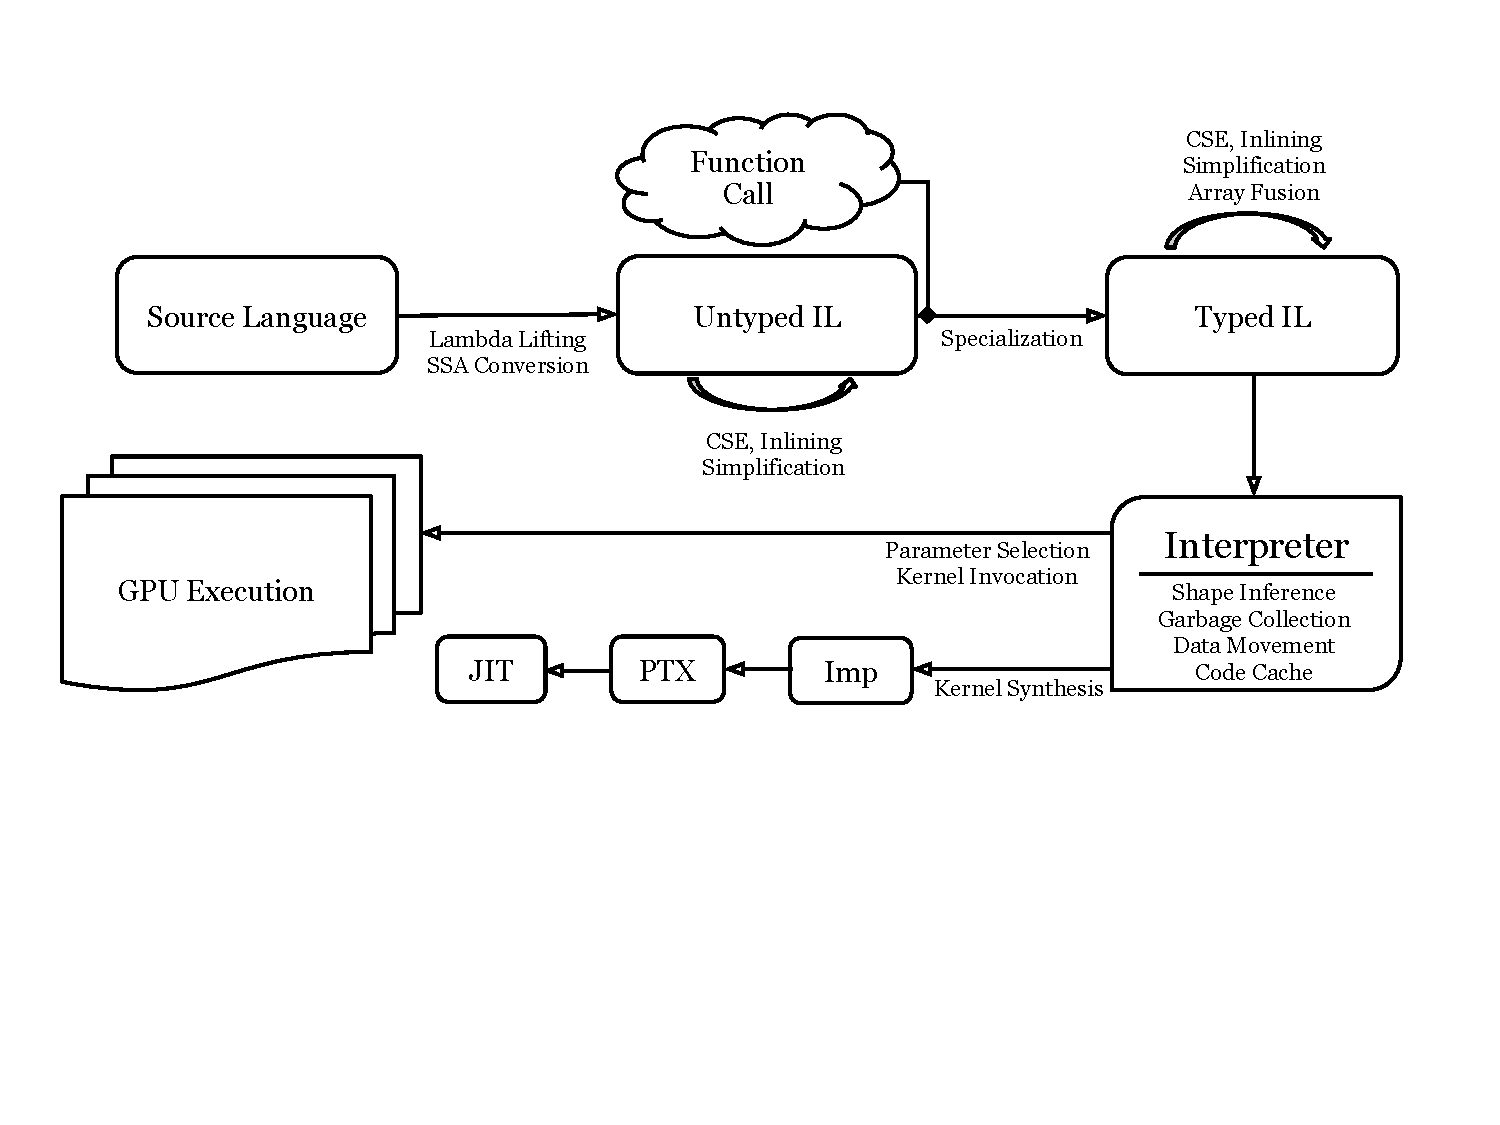
\includegraphics[scale=0.6, trim=10pt 180pt 10pt 120pt]{Pipeline.pdf}
\end{center}
\caption{Overview of Parakeet}
\label{fig:overview}
\end{figure*}
\section{Overview}
\label{overview}

As mentioned, a key target audience for Parakeet is scientific programmers. In general, the target audience includes the large majority of programmers who aren't specialists in tuning low level code to get peak performance.  The goal for Parakeet is to enable these programmers to take advantage of the acceleration potential of GPUs by automating the steps of the process that require highly specialized knowledge.

At present, a typical usage pattern in scientific computing is to prototype an algorithm in a high level interactive language such as Matlab due to the ease of rapid exploration of the problem domain in such an environment.  Then, since run times for these programs are typically on the order of hours or days, it is often necessary for performance performance reasons to port them to a high performance language such as C or CUDA.  Beyond the need for specialized high performance programming skills, a problem with this procedure  lies in the disconnect between the environment for domain exploration and the environment in which real results can be derived as it greatly hinders productivity.

Our thesis is that if we can JIT compile and transparently accelerate the critical paths of algorithms written in array-oriented languages, we can bring the best of both worlds together -- viz., the ease of use and domain exploration of the dynamic, interactive environment; and the speed of the hand optimized versions. A key constraint in such a setup is keeping JIT compilation overheads low enough so as not to impair the interactive nature of the source language environment.  It has been shown in the pioneering JIT work by Chambers~\cite{Cham92} that in such scenarios the key psychological barrier for compilation overhead is roughly on the order of less than half a second: if overheads are kept below this threshold, the programmer doesn't notice them.  Since our JIT costs are indeed low and are negligible in comparison with the run times of the large scientific codes, we feel it is reasonable to expect programmers to pay them in return for the resultant large runtime speedups so long as the JIT costs don't slow down their workflow.

\subsection{Execution Pipeline}
\label{executionpipeline}

The program execution pipeline for our system (shown in Figure \ref{fig:overview}) begins in the standard interpreter of the source array language.  Parakeet is designed as an accelerator library for dynamic, interpreted array languages, and is attached to the source language's interpreter via its plugin interface. This allows the programmer to continue to use all of the language's normal tools and support libraries.

The core of the Parakeet framework is its internal typed intermediate language and an interpreter provided for that language. This IL includes data parallel array operators such as \textbf{map}, \textbf{reduce}, and \textbf{scan} that translate well into efficient data parallel GPU programs (a full table of the supported operators can be found in Figure \ref{ArrayOps}).

Execution of a program proceeds as normal in the source language's interpreter, with Parakeet intercepting function calls.  The source of these functions is then translated into an untyped intermediate representation using the Parakeet front end interface and the source language's facilities for introspection. At this step, various standard compiler optimizations are applied to the untyped IL AST such as common subexpression elimination.

When a call is made to such an intercepted function, the untyped function body is type specialized according to its argument types.  Further standard optimizations are performed at this stage, as well as an optimization we call \emph{array operator fusion}.  Here, nested array operators are fused according to various rewriting rules into fewer operators. This fusion step can be extremely beneficial to the final GPU program's performance, as it eliminates temporaries and therefore achieves more efficient use of GPU memory bandwidth.

Next, the Parakeet interpreter interprets the typed IL version of the function.  When Parakeet reaches an array operator node in the code tree, it employs a simple cost-based heuristic (which includes things such as data size and memory transfer costs) to decide whether to execute that array operator on the GPU or CPU (for more details see Section \ref{costmodel}).  Some code simply cannot be efficiently translated into GPU programs (such as that which performs I/O or modifies global state), and such code is kept on the CPU. In the case where Parakeet executes the operator on the CPU, the operator is either (1) translated into an IL implementation and then executed by the Parakeet interpreter; or (2) passed back to the source language's interpreter for execution. In this way, we are able to support the entire source language by simply deferring to its interpreter all computation we don't wish to perform or don't yet support. The Parakeet interpreter's execution of IL code hasn't been heavily optimized as of yet -- our effort has been focused on the generation of efficient GPU kernels.  This is reasonable for now, as its IL is very dense since array operators express large computations extremely concisely.

If an array operator's computation is deemed a good candidate for GPU execution, Parakeet flattens all nested array computations within that operator into sequential loops.  This payload is then inlined into a GPU program skeleton that implements that operator.  For example, in the case of a \textbf{map} operation, Parakeet provides an efficient GPU skeleton that implements the pattern of applying the same function to each element of an array.  The flattened payload function argument to the \textbf{map} is inlined into this skeleton, and a complete GPU program is synthesized and JIT compiled.

To execute the GPU program, Parakeet first copies any of its inputs that aren't already present on the graphics card to the GPU's memory, which Parakeet treats as a managed cache of data present in the CPU's RAM.  However, unlike some systems similar to Parakeet, we do not by default preallocate the entirety of the GPU's memory.  Rather, Parakeet has a runtime flag that can enable such preallocation for better performance in dedicated compute server environments.  This is because we expect a typical use case to be in a desktop environment, where the GPU serves a double function of graphics processing and array operator acceleration.

The GPU program is then executed, with its output lazily brought back to the CPU either when it is needed or when Parakeet's GPU garbage collector reclaims its space. If a kernel's data doesn't fit on the GPU, we default to CPU execution for now.  We are currently implementing an approach to divide an array operator's execution into pieces to allow automatic execution of kernels on arbitrarily large inputs.

\section{GPU Hardware}
To set the stage and motivate the design choices of Parakeet, we discuss here some important features of modern GPU hardware.  A GPU consists of an array of tens of multiprocessors.  Within these multiprocessors are various resources such as local memories and instruction issue units that are shared among its simple cores. Since the issue units are shared, the threads running on a single multiprocessor execute instructions in lockstep -- hence the name Single Instruction Multiple Thread (SIMT) for the execution model.  The typical pattern is to issue a short program to be executed in parallel by thousands of lightweight threads that run on these hundreds of simple cores, each operating on different subsets of some input data.  With all these cores, a typical graphics card has a peak throughput of many hundreds of GFLOP/s -- an order of magnitude more than typical high end CPUs at a fraction of the cost.

SIMT differs from the more common Single Instruction Multiple Data (SIMD) model in that branching instructions are allowed whose branch conditions aren't uniformly met among threads within a single multiprocessor, allowing colocated threads to execute divergent code paths.  This improves the ease of programming a GPU, but divergent branching incurs a very expensive performance penalty as each thread effectively execute no-ops along the irrelevent code paths.  This illustrates a common point in GPGPU programming: the hardware allows for somewhat expressive programming styles, but failure to match what the hardware actually does well results in very inefficient execution.

Graphics cards have high peak memory bandwidth -- well over 100GB/sec is common.  However, in order to achieve this high bandwidth (which is essential to achieving peak performance), nearby threads must access memory in particular, regular patterns.  Random memory access can be over an order of magnitude slower than linear stride access.  To alleviate some of this performance bottleneck, the GPU also provides several other memory spaces with varying performance characteristics and preferred access patterns.  These memory spaces include some read-only cached space (called \emph{texture} and \emph{constant} memory) and some programmer-managed multiprocessor-local fast memory called \emph{shared memory}.  Efficient manual use of these memory spaces can be quite cumbersome, but is also essential to good performance for most workloads.

\subsection{Limitations Imposed by GPUs}
\label{GPULimitations}
GPUs are able to achieve their specialized high performance because they have been optimized for data parallel workloads. Data parallelism is widely found in typical graphics applications that perform simple operations on large amounts of pixel or triangle data, and so is a natural choice for execution on graphics accelerators.  However, architectural optimization for data parallelism carries with it various restrictions on the types of code and programming models that naturally fit the GPU architecture:

\begin{itemize}
\item \textbf{Flat, unboxed data representation}. GPU hardware is optimized to utilize memory in highly structured access patterns (so-called ``coalescing''). The use of boxed or indirectly accessed data leads to unstructured memory accesses and results in severe performance degradation.

\item \textbf{No polymorphism}. GPUs generally share instruction dispatch units among many concurrently executing threads. When a group of threads ``diverge'', meaning that they take different branches through a program, their execution must be serialized. Thus it is important to eliminate as many sources of runtime uncertainty as possible. In particular, type-tag dispatch commonly used to implement polymorphic operations would incur unacceptable costs if translated naively to the GPU.

\item \textbf {No function pointers}. Most GPUs (excluding the recently released NVIDIA Fermi architecture) do not support the use of indirect jumps or function pointers. In fact, a common implementation strategy for GPU function calls is extensive inlining. Even in the case where function pointers are theoretically supported, they require every possible function to be transferred to the GPU and incur overhead due to potentially unpredictable branching.

\item \textbf{No global communication}. Synchronization in a GPU computation is limited to local neighborhoods of threads. Various schemes have been devised for achieving global synchronization between all executing threads~\cite{feng10}, but these schemes are all either slow or unsafe. This implies that the use of shared mutable state is a large hindrance to effective utilization of GPU resources.

\item \textbf{All data must be preallocated}. The current generation of GPUs lack any mechanism for dynamically allocating memory. Any heap space required by a GPU computation (for output or temporary values) must be allocated beforehand.
\end{itemize}

With these constraints in mind, we turn to efficient high level abstractions chosen to fit them.

\section{Array Language Programming with Q}
\label{Q}
Array programming languages, as mentioned in Section \ref{Intro}, include native support for array creation and manipulation via bulk array operators. These array operators, such as \textbf{map}, typically have natural data parallel implementations which plays well to the strengths of GPUs.  A key contribution of Parakeet is to provide a compiler framework that capitalizes on this strength while respecting the constraints necessary to maintain good performance.

While the Parakeet framework is built to be agnostic to the source array language, we chose to implement its first front end for Q, a high-level, sequential array programming language from the APL family \cite{Borr08}. Q is dynamically typed and uses native array types and a rich set of array operators and higher-order data parallel function modifiers that map well onto the Parakeet array operators. Q is also a fully-featured language, with a large library of built-in functions, and is fast enough to support
intraday trading in the financial computing domain. Since the focus of this paper is the Parakeet runtime and compiler, we omit many details of the Q language.  We present only the salient features for illustrating the programming style and Q's support for array operators.

\subsection{K-Means Clustering Example}
\begin{figure}[h!]
\begin{lstlisting}
calc_centroid:{[X;a;i] avg X[where a = i]}
calc_centroids:{[X;a;k]
  calc_centroid[X;a] each til k}

dist:{[x;y] sqrt sum (x-y) * (x-y)}
minidx:{[x] x ? min x}

kmeans:{[X;k;a]
  C: calc_centroids[X;a;k];
  converged: 0b;
  while[not converged;
    lastAssignment: a;
    D: X dist/:\: C;
    a: minidx each D;
    C: calc_centroids[X;a;k];
    converged: all lastAssignment = a];
  C}
\end{lstlisting}
\caption{K-Means Clustering implemented in Q}
\label{QKMeans}
\end{figure}

%TODO: Insert K-Means \cite{MacQ67}
We illustrate the relevant features of array programming in Q with an example: an implementation of K-Means clustering, a widely used unsupervised clustering algorithm.  In Figure \ref{QKMeans}, we see an implementation of K-Means in Q.  Five functions are defined using Q's brace notation for surrounding function bodies and the colon operator for assignment. For example, the \texttt{calc\_centroid} function on line 1 takes three parameters \texttt{X}, \texttt{a}, and \texttt{i} (used as the input data matrix, the
current assignment vector, and the scalar index of the centroid to calculate, respectively), and calculates that cluster's current centroid.

This function illustrates some of the array-oriented features of Q. First, Q allows implicit mappings of functions elementwise across vectors -- for example, to test elementwise equality between the assignment
vector \texttt{a} and the scalar index \texttt{i}, we simply write \texttt{a = i}.  In addition, this showcases Q's support for \emph{scalar promotion}.  Semantically, Q implicitly promotes \texttt{i} to be a vector of the value of \texttt{i} repeated a number of times equal to the length of \texttt{a} and computes the elementwise equality of these two vectors.

We then generate the list of indices we want by applying the built-in \texttt{where} operator to the result of this test, and index into the data matrix \texttt{X} to get the list of data points in the centroid. The result of this indexing is itself a 2-D matrix which contains the list of data points belonging to the \texttt{i}-th cluster. Finally, the built-in \texttt{avg} function -- a reduction operator -- gets applied to this 2-D list. Thus we see that reductions and other built-in array operators can be applied to arrays of any arity.  Further array built-ins used in K-Means include \texttt{sum}, \texttt{min}, and the find operator (denoted by `\texttt{?}').

In this algorithm we also see a number of higher-order data-parallel function modifier keywords, which in Q are called \emph{adverbs}.  For example, the \texttt{each} keyword modifies a function by applying it elementwise to its argument.  In the \texttt{calc\_centroids} function, we calculate each cluster's
new centroid by using \texttt{each} to apply the \texttt{calc\_centroid} function to a list of integers from \texttt{0} to \texttt{k-1}.  The other adverbs used in K-Means are the directional each variants, \texttt{each-left} and \texttt{each-right} (denoted by \texttt{$\backslash$:} and  \texttt{/:}, respectively). These adverbs modify a binary function and apply it to each element of the respective input argument.  By combining both, we are able to apply the \texttt{dist} function to each pair of rows from the two input arrays--i.e.~to each data point and each centroid to calculate all the needed distances for reassigning the centroids.

We see that array programming languages are both expressive and compact.  While the CUDA implementation of K-Means in the Rodinia benchmark suite is hundreds of lines of code long, our Q version is only 17 even though we wrote in a verbose style in the interest of clarity. Importantly, the Q program is sequential as well.

\section{Typed Intermediate Language}
Now we turn to the problem of compiling an array language program into an efficient GPU program. At first glance, there seems to be a significant mismatch between the highly dynamic expressiveness of an array language like Q and the limitations imposed by GPU hardware discussed in Section \ref{GPULimitations}. Indeed, the Parakeet intermediate language must serve as a compromise between two competing tensions. First, in order to translate array programs into efficient GPU code it is necessary for the compiler to eliminate as much abstraction as possible. On the other hand, we must be careful not to make our program representation overly concrete with regard to evaluation order (which would eliminate opportunities for parallelism provided by the array operators).

In deference to the above-mentioned GPU hardware restrictions we disallow from our intermediate language:

\begin{itemize}
\item Polymorphism of all kinds
\item Recursion
\item User-specified higher-order functions
\item Compound data types other than arrays
\end{itemize}

These restrictions are not necessarily as severe as they initially seem, since the programmer needn't know about them. This is simply the internal format Parakeet uses in order to generate efficient GPU back end code. We explain the specialization algorithm later on in this paper.

Our intermediate language is shown in Figure \ref{ILandType}. The parallelism abstraction we prefer to maintain is the use of the higher-order array operators $\MAP$, $\REDUCE$, and $\SCAN$. The higher-order array operators form a carefully confined higher-order subset of our otherwise first-order language and thus we elevate them to primitive syntax. These operators are important since they are the only constructs in our language that we attempt to parallelize automatically through GPU code synthesis.

This isn't to say these are the only constructs executed in parallel on the GPU. The simple array operators such as \textbf{sort} (a full list can be found in Figure \ref{ArrayOps}) are executed in parallel on the GPU as well. They simply aren't higher-order, and thus are implemented via a fixed parallel standard library.

We take inspiration from \cite{Bol09} and allow functions to both accept and return multiple values. This feature simplifies the specification of certain optimizations and naturally models the simultaneous creation of multiple values on the GPU. By convention we will write $\overline{\tau_m}$ to denote a sequence of $m$ simple types, $\overline{v_n}$ for a sequence  of $n$ values, etc. A single element is equivalent to a sequence of length 1 and sequences may be concatenated via juxtaposition, such that $\tau, \overline{\tau_n} = \overline{\tau_{m+1}}$.

\begin{figure}
  \begin{tabular}{| m{0.01cm}m{1.5cm}m{0.1cm}m{0.2cm}p{4.5cm} |}
  \hline
  & & & &\\
   \multicolumn{5}{|l|}{\textbf{Intermediate Language Syntax}}  \\[4pt]
  & program & $p$ &  $\bnfdef$   &  $d_1 \cdots d_n $ \\[4pt]
  & definition & $d$ & $\bnfdef$ & $f_i(\overline{x_m} : \overline{\tau_m}) \rightarrow (\overline{y_n} : \overline{\tau_n}) =s^{\small{+}}$ \\[4pt]
  & statement  & $s$ & $\bnfdef$ & $\overline{x_m} : \overline{\rho_m} = e $\\[2pt]
  &            &     & $\sep$    & $\IF \;v\; \THEN \;s^*\; \ELSE \;s^*$ \\[2pt]
  &            &     & $\sep$    & $\WHILE \;e\; \DO \;s^+\;  $ \\[4pt]
  & expression & $e$ & $\bnfdef$ & $ v_{f}(v_1, \ldots, v_m)$ \\[2pt]
  &            &     & $\sep$    & $\textrm{values} (\overline{v_m})$ \\[2pt]
  &            &     & $\sep$    & $\textrm{cast} \; (v, \tau)$ \\[2pt] 
  &            &     & $\sep$    & $\MAP_m (v_{f},\overline{v_m})$ \\[2pt]
  &            &     & $\sep$    & $\REDUCE_m (v_{f}, v_{g}, v_{init}, \overline{v_m})$ \\[2pt]
  &            &     & $\sep$    & $\SCAN_m (v_{f}, v_{g}, v_{init}, \overline{v_m})$ \\[4pt]
  & value      & $v$ & $\bnfdef$ & numeric constant\\[2pt]
  &            &     & $\sep$    &  $x$  \quad \small{(data variable)} \\[2pt]
  &            &     & $\sep$    &  $f$  \quad \small{(function label)} \\[2pt]
  &            &     & $\sep$    &  $\oplus$ \quad \small{(scalar operator)} \\[2pt]
  &            &     & $\sep$    &  $a$ \quad \small{(simple array operator)}
\\[4pt]
  & & & &\\
  \multicolumn{5}{|l|}{\textbf{Type System}} \\[4pt]
  & data     & $\tau$    & $\bnfdef$ & $int \sep float \sep \mathbf{vec} \; \tau   $ \\[4pt]
  & closures        & $\rho$  & $\bnfdef$ & $\{f_i, \overline{\tau_{c}} \} \Rightarrow \overline{\tau_m} \rightarrow \overline{\tau_n}$\\[2pt]
  &                 &           & $\sep$    & $\tau$ \\[4pt]
  & higher-order    & $\theta$  & $\bnfdef$ & $\overline{\rho_m} \rightarrow
\overline{\rho_n} $ \\[4pt]
  & & & &\\
  \hline
  \end{tabular}\\[4pt]
\caption{Intermediate Language and Type System}
\label{ILandType}
\end{figure}

Scalar operators include the usual boolean operations as well as scalar and floating point arithmetic operators and functions. Examples of simple array operators include indexing, replication, and inspecting an array's shape.

Salient features of our intermediate language include:
\begin{itemize}
\item In order for higher-order functions to be translated into the Parakeet IL, it must be possible to specialize away all higher-order arguments. There are situations where exhaustive specialization is not possible (e.g., combinator libraries); in these cases, we revert to the source language's interpreter for
execution. This highlights an important point: since Parakeet augments (but does not replace) the interpreter of the source language, we are free to disallow problematic language constructs from Parakeet.

\item It is important to note that we can still represent function values within our intermediate language (which are created by partial application of top-level functions). However, since user functions cannot themselves accept other functions as arguments, the only purpose of function values is to parameterize the $\MAP$, $\SCAN$, and $\REDUCE$ higher-order primitives.

\item It is also worth highlighting the curious nature of the type we assign to function values:
$ \{ f_i, \overline{\tau_{c}} \} \Rightarrow \overline{\tau_m} \rightarrow \overline{\tau_n}$.  The terms occurring before the double arrow ($\{f_i, \overline{\tau_{c}} \}$) represent both the function label of a closure and the types of partially applied function arguments. We attach this information to a closure's type to facilitate efficient passing of closure arguments to the GPU and avoid any actual indirection which might otherwise be associated with function invocation. The need to statically determine a function label for any closure restricts which programs Parakeet can compile. We must reject any code where the function
that executes at a particular program point depends on some dynamic condition.
\end{itemize}

\begin{figure}
\begin{center}
\begin{tabular}{|p{2.25cm}|p{5.5cm}|}
\hline
\multicolumn{2}{|c|}{\textbf{Higher-Order Array Operators}}\\[4pt] \hline
\textbf{Array Operator} & \textbf{Meaning}\\[4pt] \hline
\textbf{map}($f$,$x$) & Apply function $f$ to all elements of $x$\\[4pt] \hline
\textbf{reduce}($f$,$init$,$x$) & Return result of inserting binary $f$ \\
& between all elements of $x$ prefixed by $init$\\[4pt] \hline
\textbf{scan}($f$,$init$,$x$) & Return running application of $f$ to $init$ \\
& and each element of $x$\\[4pt] \hline
\end{tabular}
\\[12pt]
\begin{tabular}{|p{2.25cm}|p{5.5cm}|}
\hline
\multicolumn{2}{|c|}{\textbf{Simple Array Operators}}\\[4pt] \hline
\textbf{Array Operator} & \textbf{Meaning}\\[4pt] \hline
\textbf{sort}($x$) & Return a sorted version of $x$\\[4pt] \hline
\textbf{find}($x$,$i$) & Return index of first occurence of $i$ in
$x$\\[4pt] \hline
\textbf{where}($x$) & Return an array of indices where $x$ = 1\\[4pt] \hline
\textbf{index}($x$,$i$) & Return the value of $x$ at index $i$\\[4pt] \hline

% Which other ones do we support and want to list?
\end{tabular}
\caption{Parakeet's Supported Array Operators}
\label{ArrayOps}
\end{center}
\end{figure}

\section{Translation, Specialization, and Optimization}
\label{Compilation}
In this section we describe the various program transformations we perform before executing a user's function. Some of these transformations (such as lambda lifting and specialization) are necessary in order to bridge the abstraction gap between an expressive dynamically typed language and the GPU hardware. We also demonstrate several optimizations which, while beneficial in any compiler, are particularly important when targetting a graphics processor. Seemingly small residual inefficiencies in our intermediate form can later manifest themselves as the creation of large arrays, needless memory transfers, or wasteful GPU computations.

To help elucidate the different program transformations performed by Parakeet, we will show the effect of each stage on a distance function defined in Q, shown in Figure \ref{QDist}.

\begin{figure}[h!]
    \begin{lstlisting}[numbers=none]
    dist: {[x;y] sqrt sum (x-y) * (x-y)}
    \end{lstlisting}
    \caption{Distance Function in Q}
    \label{QDist}
\end{figure}

\subsection{Lambda Lifting and SSA Conversion}
After a function call has been intercepted by the Parakeet runtime, Parakeet performs a syntax-directed translation from a language-specific abstract syntax tree (AST) into Parakeet's IL. Since type information is not yet available to specialize user functions, the functions must be translated into an untyped
form (by setting all type assignments to $\bot$). The translation into Parakeet's IL maintains a closure environment and a name environment so that simultaneous lambda lifting and SSA conversion can be performed.
% What does SSA conversion mean? We should define.

Since we would like to interpret our intermediate language we use a gated SSA form based on the GSA sub-language of the Program Dependence Web \cite{Ott90}. Classical SSA cannot be directly executed since the $\phi$-nodes lack deterministic semantics. Gated SSA overcomes this limitation by using "gates" which not only merge data flow but also associate predicates with each data flow branch. Aside from simplifying certain optimizations, these gates also enable us to execute our code without converting out of SSA.  Figure \ref{UntypedSSADist} shows the \texttt{dist} function after it has been translated to Untyped SSA.

\begin{figure}[h!]
\fbox{
\begin{tabular}{ m{0.1cm} m{6.7cm} }
  \multicolumn{2}{l}{dist $($ x, y $) \rightarrow  ($ z $) =$} \\
  & t$_1 = \mathrm{x} - \mathrm{y} $        \\
  & t$_2 = \mathrm{x} - \mathrm{y} $        \\
  & t$_3  = \mathrm{t}_1 * \mathrm{t}_2 $   \\
  & t$_4  = $sum$(\mathrm{t}_2) $           \\
  & z $  = \; \mathrm{sqrt}(\mathrm{t}_4)$   \\
\end{tabular}
}
\caption{Untyped Distance Function in SSA form}
\label{UntypedSSADist}
\end{figure}

\subsection{Untyped Optimizations}
Parakeet performs optimizations both before and after type specialization. We subject the untyped representation to inlining, common subexpression elimination and simplification (which consists of simultaneous constant propagation and dead code elimination). This step occurs once for each function, upon its first interception by Parakeet. It is preferable to eliminate as much code as possible at this early stage since an untyped function body serves as a template for a potentially large number of future specializations. The only optimizations we do not perform on the untyped representation are array fusion rewrites, since these rely on type annotations to ensure correctness.

In our distance example, untyped optimizations will both remove a redundant subtraction and inline the definition of the $sum$ function, which expands to a $\REDUCE$ of addition.
\begin{figure}[h!]
\fbox{
\begin{tabular}{ m{0.1cm} m{6.7cm} }
  \multicolumn{2}{l}{dist $($ x, y $) \rightarrow  ($ z $) =$} \\
  & t$_1 = \mathrm{x} - \mathrm{y} $        \\
  & t$_2  = \mathrm{t}_1 * \mathrm{t}_1 $   \\
  & t$_3  = \REDUCE(+, 0, \mathrm{t}_2) $    \\
  & z $  = \; \mathrm{sqrt}(\mathrm{t}_3)$   \\
\end{tabular}
}
\caption{Distance Function after untyped optimizations}
\end{figure}

\subsection{Specialization}
The purpose of specialization is to eliminate polymorphism, to make manifest all implicit behavior (such as coercion and scalar promotion), and to assign simple unboxed types to all data used within a function body. Beyond the fact that the GPU requires its programs to be statically typed, these goals are all essential for the efficient execution of user code on the GPU. Thus, the specializer generates a different specialized version of a function for each distinct call string, with all of the function's
variables receiving the appropriate types.

The signature of data is one of our built-in dynamic value types such as $float$ or $vec~vec~int$.  The signature of functions is a closure that includes a function tag and a list of data signatures.  It is important to note that specialization is thus not just on types, but also on function tags and the types of their associated closure arguments. This is equivalent to performing defunctionalization (Reynolds) and
then specializing exhaustively on the constant values of closure records. One caveat here is that non-constant closure values are disallowed.  This prevents us from having to implement them as large switch statements on the GPU, which would be very inefficient due to branch divergence.  Finally, only data is
allowed to cross the boundary from our system to the source language -- specialized Parakeet functions remain enclosed in our runtime.

To continue the example, if the \textit{dist} function is called with arguments of type $vec~ float$ the specializer will then generate the code shown in Figure \ref{SpecDist}.

\begin{figure}[h!]
\fbox{
  \begin{tabular}{m{0.1cm} m{6.7cm}}
    \multicolumn{2}{l}{dist $($ x $ : vec \; float $, y : $ vec \; float $) $
\rightarrow  ($ z $ : float ) =$}  \\
    & t$_1   = \MAP ( -_{\mathrm{float}}, \mathrm{x}, \mathrm{y})$   \\
    & t$_2   = \MAP (*_{\mathrm{float}}, \mathrm{x}, \mathrm{y})$    \\
    & t$_3 = \REDUCE (+_{\mathrm{float}}, 0, \mathrm{t}_2)$          \\
    & z $  = \; \mathrm{sqrt}(\mathrm{t}_3)$                         \\
  \end{tabular}
}
\caption{Distance Function After Specialization}
\label{SpecDist}
\end{figure}

The actual intermediate language associates type annotations with every binding, which we elide here for clarity. Note that the polymorphism inherent in math operations between dynamically typed values has been removed through the use of statically typed math operators, and implicit \textbf{map}s on vectors (such as the subtraction between $x$ and $y$) have been expanded and made explicit.

\subsection{Array Operator Fusion}
In addition to standard compiler optimizations (such as constant folding, function inlining, and common sub-expression elimination), we employ fusion rules~\cite{Jones01} to combine array operators. Fusion enables us to minimize kernel launches, boost the computational density of generated kernels, and avoid the generation of unnecessary array temporaries.

We present the fusion rules used by Parakeet in simplified form, such that array operators only consume and produce a single value. Our rewrite engine actually generalizes these rules to accept functions of arbitrary input and output arities.
\\[5pt]
\begin{tabular}{|m{0.001cm} m{0.05cm} p{6.75cm} p{0.05cm} |}
  \hline 
  & &  & \\
  & \multicolumn{2}{l}{\large{Map Fusion} }  &  \\[2.5pt]
  & & $\MAP(g, \MAP(f, x)) \leadsto \MAP(g \circ f, x)$ & \\
  & & & \\
  & \multicolumn{2}{l}{\large{Reduce-Map Fusion} }  & \\[2.5pt]
  & & $\REDUCE(g_r, g_{i}, \MAP(f, x)) \leadsto \REDUCE(g_r \circ f, g_{i} \circ f, x)$ & \\
  & & & \\
  \hline
\end{tabular}\\[4pt]
These transformations are safe if the following conditions hold:
\begin{enumerate}
\item All the functions involved are referentially transparent.

\item Every output of the predecessor function ($f$) is used by the successor
($g$).

\item The outputs of the predecessor are used \textit{only} by the successor.
\end{enumerate}
The last two conditions restrict our optimizer from rewriting anything but linear chains of produced/consumed temporaries. A large body of previous work~\cite{Ald01} has demonstrated both the existence of richer fusion rules and cost-directed strategies for applying those rules in more general scenarios. Still, despite the simplicity of our approach, we have observed that many wasteful temporaries in idiomatic array code are removed by using only the above rules.

In Figure \ref{DistFuse}, we see the resulting optimized and specialized \texttt{dist} function. The two \textbf{map}s have been fused into the \textbf{reduce} operator, with a new function $f_1$ generated to perform the computation of all three original higher-order operators.

\begin{figure}[h!]

\fbox{
  \begin{tabular}{m{0.1cm} m{6.7cm} }
    \multicolumn{2}{l}{$\mathrm{f}_1 ($ acc : $ float $,  x $ : float $, y : $ float $) $ \rightarrow  ($ z $ :  float ) =$} \\
    & t$_1 = x - y $            \\
    & t$_2  = t_1 * t_1 $       \\
    & z $ = $ acc $+$ t$_2$     \\
    &  \\ 
  \multicolumn{2}{l}{$\mathrm{dist} ($~x $ : vec \; float $, y : $ vec \; float
$) $ \rightarrow  ($ z $ : float ) =$} \\
  & t$_3 = \REDUCE (\mathrm{f}_1, 0.0, \mathrm{x}, \mathrm{y})$   \\
  & z $ = \mathrm{sqrt}(\mathrm{t}_3)$  \\
  \end{tabular}
}
\caption{Distance Function After Fusion Optimization}
\label{DistFuse}
\end{figure}

\section{The Parakeet Runtime and Implementation}
\label{runtime}

In this section, we discuss the internals of the Parakeet runtime in more detail. We implemented the Parakeet runtime and intepreter in OCaml due to its amenability to compiler writing.  We spent considerable effort tuning the OCaml code to be efficient and to prevent OCaml's garbage collector from becoming a source of large overheads. The intepreter uses an interface written in C to allow it to interact with CUDA and with NVIDIA's GPU JIT compiler.  Parakeet also exposes a front end interface written in C for translating functions from the source language into Parakeet ASTs and to pass data between the source language's interpreter and the Parakeet runtime.

When a function call is made to a function registered with Parakeet, the Parakeet interpreter intercepts the call and type specializes the function for the argument types passed in. The interpreter then walks this typed IL version of the function.  When it encounters a simple scalar math operation, the standard behavior is simply to execute that operation itself.  Any I/O or other operations that aren't supported by Parakeet's IL are simply executed by the source language's interpreter.

\subsection{Cost Model}
\label{costmodel}

When the Parakeet interpreter encounters an array operator, it uses a simple cost model to decide what is the best place to execute the operator.  The cost model employs a recursive function that estimates the relative cost of executing that operator on the CPU versus the GPU.  This function is not meant to measure the precise expected run time of the operator; rather, the goal is to make the correct decision when the use of one or the other processor should result in much higher performance.  We use the clock frequency of each processor to roughly estimate the cost of a single operation.  For each array operator, we multiply the estimated cost of a single execution of the operator's function argument by some fixed function of the input size.  For a \textbf{map} operation, for example, we multiply the estimated cost of performing the sequentialized version of the mapped function by the number of input elements. In addition, we estimated the time needed to transfer data to and from the GPU as a function of data size and add this cost to the total if the data is not already present in the respective processor's memory.

In the case of nested array operators -- e.g.~a \textbf{map} whose payload function is itself a \textbf{reduce} (as is present in the \texttt{calc\_centroids} function in the K-Means benchmark, where the \textbf{avg} reduction is mapped over each centroid index) -- the interpreter needs to choose which operator, if any, will form the parallelization point for a GPU kernel while sequentializing all nested operators within that kernel.  The possible choices include:

\begin{enumerate}
\item Running the \textbf{map} as a GPU kernel, with an embedded sequential \texttt{for} loop that implements the \textbf{reduce}.
\item Running the \textbf{map} as a \texttt{for} loop in the Parakeet interpreter, with each iteration of the loop calling a GPU kernel that implements the \textbf{reduce}.
\item Running everything in the Parakeet interpreter as two nested \texttt{for} loops.
\item Running everything in the source language's interpreter.
\end{enumerate}

In cases (1), (3), and (4), the operator is executed entirely on a single processor.  In case (2), however, the \textbf{map} runs as a loop on the CPU, generating each element of the resulting vector with a separate GPU program invocation.  In this case, the interpreter creates an interpreter array object on the CPU whose elements are references to the values generated on the GPU.  The final linear CPU array is only constructed lazily as needed or when the GPU garbage collector needs the space.  At that point, a lineary CPU array is allocated and filled in with the computed values.  This is precisely what happens in our implementation of K-Means clustering discussed in Section \ref{results-k-means}.

\subsection{GPU Back End}
Our GPU back end only supports NVIDIA GPUs at the moment due to our use of various NVIDIA-specific constructs. NVIDIA GPUs are typically programmed using CUDA, a C API for writing and executing GPU programs. In CUDA, a program is organized into {\it kernels} and {\it host} code. Kernels are executed on the GPU by typically many thousands of lightweight threads.  Host code is the name for the code run on the CPU. Typically, a host thread acts as a master that asynchronously launches worker kernels onto the GPU via function calls to the CUDA API.  The host thread in our case is simply the Parakeet interpreter itself.

Unlike many other systems similar to Parakeet, our back end doesn't emit CUDA code to be compiled by the NVIDIA CUDA compiler.  Instead, we emit PTX, NVIDIA's GPU pseudoassembly language.  (As we will see in the following section, we also have one additional level of intermediate language, which we call Imp, to which the typed IL discussed in Section \ref{Compilation} is translated before it in turn gets translated to PTX code.)  The PTX code is JIT compiled by the NVIDIA graphics driver before being executed.  We keep these compiled binary GPU versions of functions in a code cache so that when they are invoked multiple times with the same argument types we needn't incur the code generation and JIT compilation costs more than once.

The reason that we emit PTX instead of CUDA code is largely our latency requirements, as our goal is to provide a framework for transparent acceleration of interactive languages. The NVIDIA CUDA compiler is a wrapper around the GCC C++ compiler, and CUDA supports all of C++ in the host code and a large subset (including C++ templates) in the GPU code.  Thus, the compile times for even simple kernels can be on the order of 5--10 seconds.  There are, of course, advantages to using the NVIDIA compiler. The main ones are that we would be able to take advantage of all of the NVIDIA and GCC compiler optimizations and that it would simplify our implementation effort.  However, the strict latency requirements meant that we needed to emit PTX directly.

\subsection{Imp}
\label{Imp}

As mentioned above, we implement the higher-order array operators as skeletons of code with splice points where their payload functions get inlined.  Rather than implement these skeletons directly in CUDA or PTX, Parakeet includes a second intermediate language that we call Imp (short for imperative) which we use for this purpose.  This means in addition that in order to inline a function into a higher-order Imp skeleton we must first translate the function's body from the higher level Parakeet IL into Imp.

Imp is largely a syntactic sugar wrapper around PTX that simplifies our job of implementing efficient GPU versions of these operator skeletons by hiding some of the architectural details PTX exposes. Imp differs from PTX in the following important respects:

\begin{enumerate}
\item  Arrays are not associated with a particular GPU memory space (global, texture, constant, etc..), allowing us to compile variants of an Imp kernel where inputs reside in different memory spaces.

\item Space requirements of a function call (all outputs and local arrays it must allocate) can be determined as a function of input sizes. This is necessary as GPU computations have access only to memory which is allocated before their launch and cannot ``dynamically'' allocate more memory.

\item Local temporaries can be arrays in addition to scalars. This generalizes CUDA's use of ``local'' memory for spilled scalar variables.
\end{enumerate}
Imp kernels are ``shapely'' by construction, meaning they specify their memory requirements as deterministic functions of input size. This obviates the need for ad-hoc allocation logic (the bulk of most CUDA host code in practice) or for auxiliary size inference on higher level code. If a function can be translated to Imp then we can always determine its memory requirements.

We perform staged synthesis of Imp kernels by parameterizing them with payload functions. An Imp kernel can be seen as a ``skeleton'' \cite{Cole04} for a particular implementation strategy of some array operator. In reality, we don't actually program directly in Imp.  Rather, we use Imp as an embedded DSL in our OCaml Parakeet code.  We then use OCaml as a meta-language that programmatically constructs an Imp version of the array operator with the payload function inlined.

An example of a simplified Imp skeleton for \textbf{map} is shown in Figure \ref{ImpMap}.  The lines with the \texttt{SPLICE} keyword are the points at which the payload function gets added to the skeleton to form a complete kernel.

\begin{figure}[h!]
  \begin{lstlisting}[numbers=none]
    
  \end{lstlisting}
  \caption{Imp Map Skeleton}
  \label{ImpMap}
\end{figure}

\subsection{Shape Inference}
\label{shapeinference}

Alex should write a couple paragraphs about how he does shape inference here.

\subsection{Parallel Library}

In addition to these skeletons, we provide a library of precompiled parallel implementations of our simple (first-order) array operators, which are listed in Figure \ref{ArrayOps}.  Since these operators don't require synthesis with embedded payload functions, we needn't dynamically generate them.  We use the Thrust library \cite{Hobe10} for some of these operators such as \textbf{sort}, while providing our own hand-tuned implementations of others such as \textbf{where}.

\section{Evaluation}
\label{Evaluation}

We evaluated Parakeet on two standard benchmark programs: Black-Scholes option pricing, and K-Means Clustering.  We compare Parakeet against both hand-tuned CPU and GPU implementations.  For Black-Scholes, the CPU implementation is taken from the PARSEC \cite{Bien08} benchmark suite -- which we used as the basis
of our Q implementation -- and the GPU implementation is taken from the CUDA SDK \cite{NvidSD}.  For K-Means Clustering, we wrote our own Q version in 17 lines of code.  Both the CPU and GPU benchmark version come from the Rodinia benchmark suite \cite{Che09}.

Our experimental setup is as follows.  We ran the CPU benchmarks on a machine with an Intel Nehalem 2.67GHz X5550 4-core CPU with 24GB of RAM.  The theoretical peak throughput of this machine is 85.12 GFLOP/s, and it has a theoretical peak memory bandwidth of 32GB/s.

For all GPU benchmarks, we ran the programs on an NVIDIA GTX260. This card has 216 processor cores with clock speeds of 1.3 GHz and 896MB of memory, with peak execution throughput of 805 GFLOP/s and peak memory bandwidth of 112 GB/s.

For all of our Parakeet benchmarks, the desktop system we used for running the interpreter had an Intel Core 2 6600 2.4GHz processor with 2 cores and 4GB of RAM.

\subsection{Black-Scholes}
\label{results-bs}

Black-Scholes option pricing \cite{Blac73} is a standard benchmark for data parallel workloads, since it is embarrassingly parallel -- the calculation of the price of a given option doesn't impact that of any other, and the benchmark consists of simply running thousands of independent threads in parallel for computing the prices of thousands of options.

We compare our system against the multithreaded OpenMP CPU implementation from the PARSEC \cite{Bien08} benchmark suite with 4 threads and the CUDA version in the NVIDIA CUDA SDK \cite{NvidSD}.

\begin{figure}
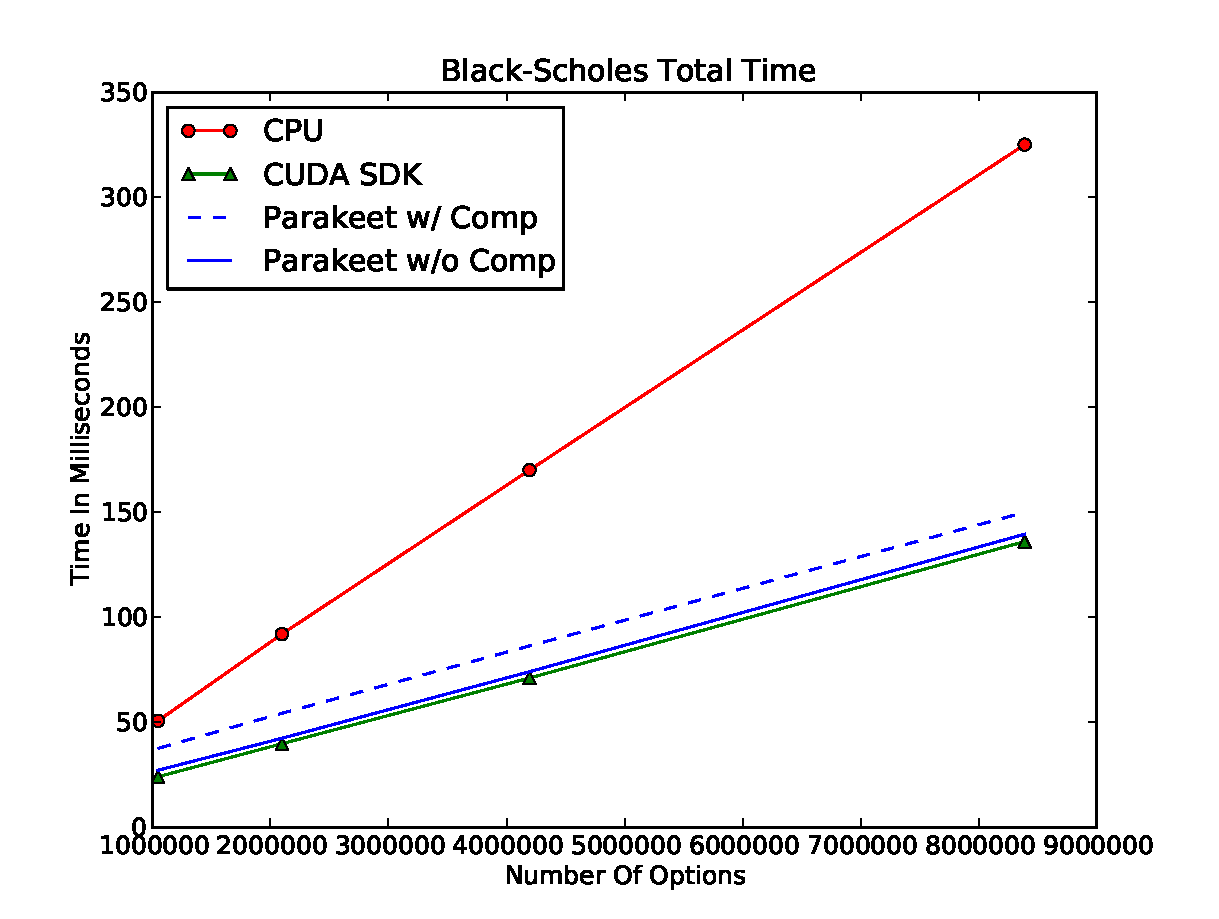
\includegraphics[scale=0.45]{BSTotal.pdf}
\caption{Black Scholes Total Times}
\label{BSResults}
\end{figure}

In Figure \ref{BSResults}, we see the total run times of the various systems. These times include the time it takes to transfer data to and from the GPU in the GPU benchmarks.  

\begin{figure}
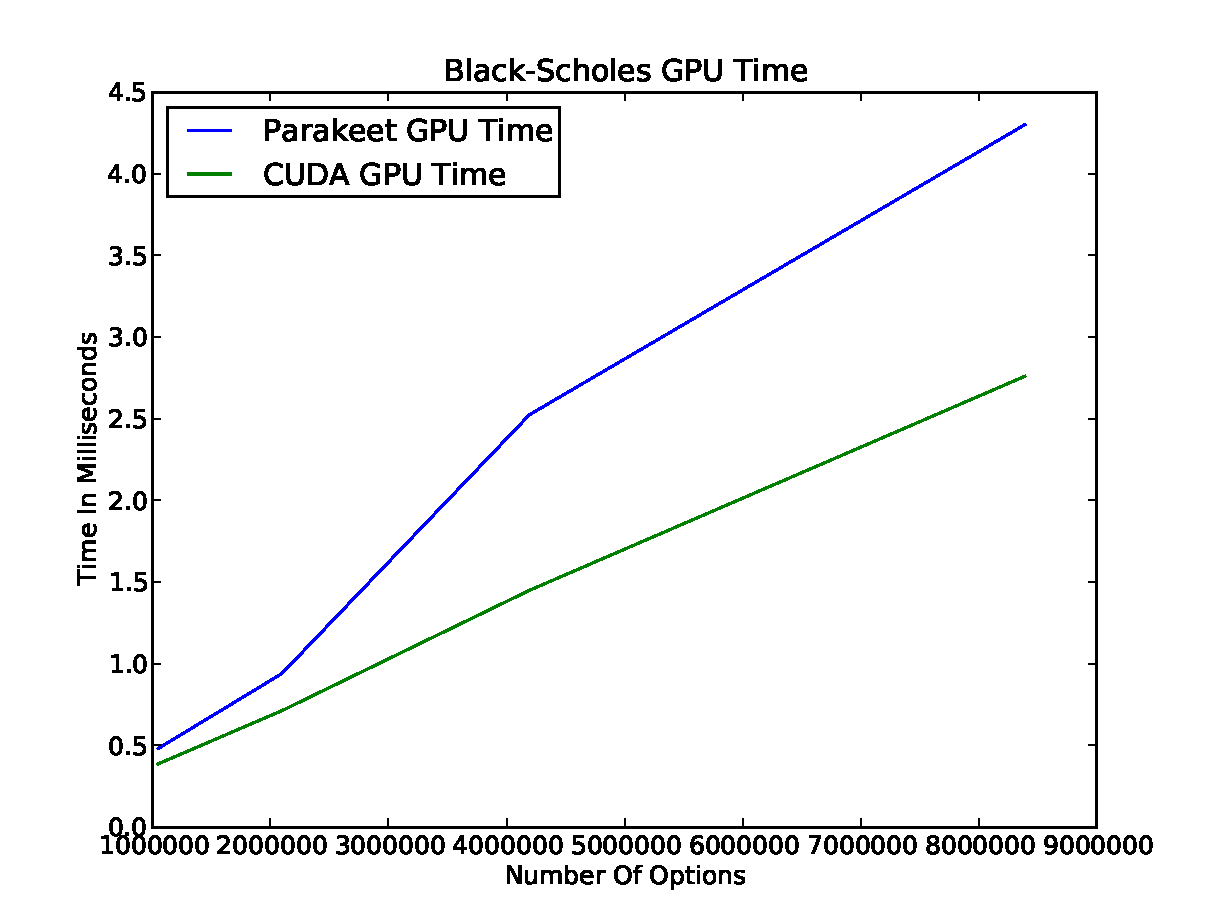
\includegraphics[scale=0.45]{BSGPU.pdf}
\caption{Black Scholes GPU Execution Times}
\label{BSResults}
\end{figure}

\subsection{K-Means Clustering}
\label{results-k-means}

K-Means illustrates a key aspect of our approach: the ability to exploit dynamic information to tailor code generation and execution.  In the \texttt{calc\_centroids} function, we have a $\MAP$ operator applied to a
nested function that in turns contains array operators.  Our interpreter is able to make the most efficient choice regarding where to execute things: the outer $\MAP$, since it's applied to a small array of integers and involves little computation of its own, gets executed on the CPU as a loop.  The inner function, which since it has dense computation applied to large inputs, gets synthesized into a kernel that is repeatedly launched.  This type of dynamic decision based on data size would not be possible in a static environment.

\section{Related Work}
\label{RelatedWork}
The use of graphics hardware for non-graphical computation has a  long history~\cite{Lengyel90}, though convenient frameworks for general purpose GPU programming have only recently emerged. The first prominent GPU backend for a general purpose language was ``Brook for GPUs'' \cite{Buck04}. The Brook language extended C with ``kernels'' and ``streams'', exposing a programming model similar to what is now found in CUDA and OpenCL.

Microsoft's Accelerator~\cite{Tard06} was the first project to use high level (collection-oriented) language constructs as a basis for GPU execution. Accelerator is a declarative GPU language embedded in C\# which creates a directed acyclic graph of LINQ operations -- such as filtering, grouping, and joining -- and compiles them to (pre-CUDA) shader programs. Accelerator's programming model does not support function abstractions (only expression trees) and its only underlying parallelism construct is limited to the production of $\MAP$-like kernels.

Four more recent projects all translate domain specific embedded array languages to CUDA backends:
\begin{itemize}
\item \textbf{Nikola}~\cite{Main10} is a first-order array-oriented language embedded within Haskell. Nikola provides a convenient syntax for expressing single-kernel computations, but requires the programmer to manually coordinate computations which require multiple kernel launches. Nikola also does not support partially applied functions and its parallelization scheme, which first serializes array operators into loops and then parallelizes loop iterations, seems ill-suited for complex array operations.

\item \textbf{Accelerate}~\cite{ChakAcc} is also an embedded array language within Haskell. Unlike Nikola, Accelerate does allow the expression of computations which span multiple kernel launches. Accelerate also has a much richer set of array operators (including the higher-order trio $\MAP$, $\REDUCE$, $\SCAN$). Accelerate, however, does not seem to support closures or the nesting of array operators. Accelerate's backend is similar to ours in that they use a simple interpreter whose job is to initiate skeleton-based kernel compilation, transfer data to and from the GPU, and to perform simple CPU-side computations.

\item \textbf{OptiML and Delite}~\cite{Chaf11} are a domain-specific language and runtime framework designed to 

\item \textbf{Copperhead}~\cite{Cata10} parallelizes a statically typed purely functional array subset of Python through the dynamic compilation/execution of CUDA kernels. Copperhead supports nested array computations, and even has a sophisticated notion of where these computations can be scheduled. In addition
to sequentializing nested array operators within CUDA kernels (as done in Parakeet), Copperhead can also share the work of a nested computation between all the threads in CUDA block. Unfortunately, Copperhead does not utilize any dynamic information (such as size) when making these scheduling decisions and
thus must rely on user annotations. Copperhead's compiler generates kernels through parameterization of operator-specific C++ template classes. By using C++ as their backend target, Copperhead has been able to easily integrate the Thrust ~\cite{Hobe10} GPGPU library and to offload the bulk of their code optimizations onto a C++ compiler. Runtime generation of templated C++ can, however, be a double-edged sword. Copperhead experiences the longest compile times of any project mentioned here (orders of magnitude longer than the compiler overhead of Parakeet).
\end{itemize}
Unlike the four approaches mentioned above, Parakeet does not require its source language to be purely functional nor statically typed. Being able to program in a dynamically typed language seems particularly important for array computations, since static type systems are generally unable to support the syntactic conveniences which make array programming appealing in the first place.

\section{Conclusion}
\label{Conclusion}

Parakeet allows the programmer to write in a high level sequential array language. Parakeet automatically synthesizes GPU programs from the resulting program and executes by transparently moving data back and
forth to the GPU's memory and performing GPU memory garbage collection. Parakeet includes a series of optimizations to generate more efficient GPU programs, including array operator fusion and the use of shared and texture memory on the GPU.  Parakeet is system in which complex programs can be written and executed efficiently.  On two benchmark programs, Parakeet delivers performance competitive with even hand-tuned CPU and GPU implementations.

In future work, we hope to support more front ends and back ends.  At the moment, we are building front ends for both Matlab and Python.  We envision building a back end for multicore CPUs as well, likely targeting LLVM~\cite{Latt02}.

In addition, we plan to increase efficiency by iteratively tuning components of hierarchical algorithms, splitting data inputs to take advantage of more of the texturing hardware, and overlapping computation with data transfer.

\bibliographystyle{acm}
\bibliography{../Parallelism}{}

\end{document}
